% !TeX program = xelatex
%% 부득이하게 pdflatex을 사용해야 할 경우 위의 magic comment를 제거하십시오.

%%%%%%%%%%%%%%%%%%%%%%%%%%%%%%%%%%%%%%%%%%%%%%%%%%%%%%%%%%%%%%%%%%%%%%%%%%%%%%%%%
%%%  LaTeX document class of the thesis of the Gyeonggi Science High School   %%%
%%%  Last edition 2015.11.13 by Chinook Mok                                   %%%
%%%  Continously being modified by gshslatexintro after 2016.02.02.           %%%
%%%  Check the latest version at : latex.gs.hs.kr                             %%%
%%%  Also refer to https://www.facebook.com/gshstexsociety                    %%%
%%%%%%%%%%%%%%%%%%%%%%%%%%%%%%%%%%%%%%%%%%%%%%%%%%%%%%%%%%%%%%%%%%%%%%%%%%%%%%%%%

\documentclass{gshs_thesis}

\graphicspath{{images/}}
% 이곳에 필요한 별도의 패키지들을 적어넣으시오.
%\usepackage{...}
\usepackage{verbatim} % for commment, verbatim environment
\usepackage{spverbatim} % automatic linebreak verbatim environment
\usepackage{listings}
\lstset{
	%basicstyle=\scriptsize,
	basicstyle=\fontfamily{NanumGothic_Coding},
	columns=flexible,
	breaklines=true
	tabsize=4, 
	numbers=left, 
	keywordstyle=\color{blue},
	extendedchars=true,    
	frame=single,	 
	keepspaces=true, 
	commentstyle=\color{magenta}
}

\usepackage{hologo}
\usepackage{booktabs}
\usepackage{listings}
\usepackage{color}
\usepackage{multirow}

\usepackage{tikz}
\usepackage{pgfplots}
\usetikzlibrary{patterns}

\usepackage{hyperref}
\hypersetup{%
	pdfborder = {0 0 0},
	colorlinks,
	citecolor=black,
	filecolor=black,
	linkcolor=black,
	urlcolor=black
}


% -----------------------------------------------------------------------
%                   이 부분은 수정하지 마시오.
% -----------------------------------------------------------------------
\titleheader{졸업논문청구논문}
\school{과학영재학교 경기과학고등학교}
\approval{위 논문은 과학영재학교 경기과학고등학교 졸업논문으로\\
졸업논문심사위원회에서 심사 통과하였음.}
\chairperson{심사위원장}
\examiner{심사위원}
\apprvsign{(인)}
\korabstract{초 록}
\koracknowledgement{감사의 글}
\korresearches{연 구 활 동}

%: ----------------------------------------------------------------------
%:                  논문 제목과 저자 이름을 입력하시오
% ----------------------------------------------------------------------
\title{NOAA/AVHRR 자료를 이용한 한반도 주변 해역의 해수면 온도 산출} %한글 제목
\engtitle{Estimation of Sea Surface Temperature around the Korean Peninsula Using NOAA/AVHRR Data} %영문 제목
\korname{박 서 진} %저자 이름을 한글로 입력하시오 (글자 사이 띄어쓰기)
\engname{Park, Seo Jin } %저자 이름을 영어로 입력하시오 (family name, personal name)
\chnname{} %저자 이름을 한자로 입력하시오 (글자 사이 띄어쓰기)
\studid{19039} %학번을 입력하시오

%------------------------------------------------------------------------
%                  심사위원과 논문 승인 날짜를 입력하시오
%------------------------------------------------------------------------
\advisor{Park, Kiehyun}  %지도교사 영문 이름 (family name, personal name)
\judgeone{김 학 성} %심사위원장
\judgetwo{이    호}   %심사위원1
\judgethree{박 기 현} %심사위원2(지도교사)
\degreeyear{2022}   %졸업 년도
\degreedate{2021}{8}{3} %논문 승인 날짜 양식

%------------------------------------------------------------------------
%                  논문제출 전 체크리스트를 확인하시오
%------------------------------------------------------------------------
\checklisttitle{[논문제출 전 체크리스트]} %수정하지 마시오
\checklistI{1. 이 논문은 내가 직접 연구하고 작성한 것이다.} %수정하지 마시오
% 이 항목이 사실이라면 다음 줄 앞에 "%"기호 삽입, 다다음 줄 앞의 "%"기호 제거하시오
%\checklistmarkI{$\square$}
\checklistmarkI{$\text{\rlap{$\checkmark$}}\square$}
\checklistII{2. 인용한 모든 자료(책, 논문, 인터넷자료 등)의 인용표시를 바르게 하였다.} %수정하지 마시오
% 이 항목이 사실이라면 다음 줄 앞에 "%"기호 삽입, 다다음 줄 앞의 "%"기호 제거하시오
%\checklistmarkII{$\square$}
\checklistmarkII{$\text{\rlap{$\checkmark$}}\square$}
\checklistIII{3. 인용한 자료의 표현이나 내용을 왜곡하지 않았다.} %수정하지마시오
% 이 항목이 사실이라면 다음 줄 앞에 "%"기호 삽입, 다다음 줄 앞의 "%"기호 제거하시오
%\checklistmarkIII{$\square$}
\checklistmarkIII{$\text{\rlap{$\checkmark$}}\square$}
\checklistIV{4. 정확한 출처제시 없이 다른 사람의 글이나 아이디어를 가져오지 않았다.} %수정하지 마시오
% 이 항목이 사실이라면 다음 줄 앞에 "%"기호 삽입, 다다음 줄 앞의 "%"기호 제거하시오
%\checklistmarkIV{$\square$}
\checklistmarkIV{$\text{\rlap{$\checkmark$}}\square$}
\checklistV{5. 논문 작성 중 도표나 데이터를 조작(위조 혹은 변조)하지 않았다.} %수정하지 마시오
% 이 항목이 사실이라면 다음 줄 앞에 "%"기호 삽입, 다다음 줄 앞의 "%"기호 제거하시오
%\checklistmarkV{$\square$}
\checklistmarkV{$\text{\rlap{$\checkmark$}}\square$}
\checklistVI{6. 다른 친구와 같은 내용의 논문을 제출하지 않았다.} %수정하지 마시오
% 이 항목이 사실이라면 다음 줄 앞에 "%"기호 삽입, 다다음 줄 앞의 "%"기호 제거하시오
%\checklistmarkVI{$\square$}
\checklistmarkVI{$\text{\rlap{$\checkmark$}}\square$}
 % usepackage 등의 명령어는 여기에.


\usepackage{tocloft}
\setlength{\cftbeforesecskip}{0pt}
\setlength{\cftbeforesubsecskip}{0pt}
\setlength{\cftbeforesubsubsecskip}{0pt}

\begin{document}

%	\renewcommand\baselinestretch{1.2} % line spacing in the paragraph
	\baselineskip=2.2em         % line spacing in the paragraph
	
	\maketitle  % command to print the title page with above variables
\setcounter{page}{1}
%---------------------------------------------------------------------
%                  영문 초록을 입력하시오
%---------------------------------------------------------------------
\begin{abstracts}     %this creates the heading for the abstract page
	\addcontentsline{toc}{section}{Abstract}  %%% TOC에 표시
	\noindent{
		Put your abstract here. It is completely consistent with 
		한글초록.
	}
\end{abstracts}

%---------------------------------------------------------------------
%                  국문 초록을 입력하시오
%---------------------------------------------------------------------
\begin{abstractskor}        %this creates the heading for the abstract page
	\addcontentsline{toc}{section}{초록}  %%% TOC에 표시
	\noindent{
		초록(요약문)은 가장 마지막에 작성한다. 연구한 내용, 즉 본론부터 
		요약한다. 서론 요약은 하지 않는다. 대개 첫 문장은 연구 주제 
		(+방법을 핵심적으로 나타낼 수 있는 문구: 실험적으로, 
		이론적으로, 시뮬레이션을 통해)를 쓴다. 다음으로 연구 방법을 
		요약한다. 선행 연구들과 구별되는 특징을 중심으로 쓴다. 뚜렷한 
		특징이 없다면 연구방법은 안써도 상관없다. 다음으로 연구 결과를 
		쓴다. 연구 결과는 추론을 담지 않고, 객관적으로 서술한다. 
		마지막으로 결론을 쓴다. 이 연구를 통해 주장하고자 하는 바를 
		간략히 쓴다. 요약문 전체에서 연구 결과와 결론이 차지하는 비율이 
		절반이 넘도록 한다. 읽는 이가 요약문으로부터 얻으려는 정보는 
		연구 결과와 결론이기 때문이다. 연구 결과만 레포트하는 논문인 
		경우, 결론을 쓰지 않는 경우도 있다.
	}
\end{abstractskor}


%----------------------------------------------
%   Table of Contents (자동 작성됨)
%----------------------------------------------
\cleardoublepage
\addcontentsline{toc}{section}{Contents}
\setcounter{secnumdepth}{3} % organisational level that receives a numbers
\setcounter{tocdepth}{3}    % print table of contents for level 3
\baselineskip=2.2em
\tableofcontents


%----------------------------------------------
%     List of Figures/Tables (자동 작성됨)
%----------------------------------------------
\cleardoublepage
\clearpage
\listoftables
% 표 목록과 캡션을 출력한다. 만약 논문에 표가 없다면 이 위 줄의 맨 앞에 
% `%' 기호를 넣어서 주석 처리한다.

\cleardoublepage
\clearpage
\listoffigures
% 그림 목록과 캡션을 출력한다. 만약 논문에 그림이 없다면 이 위 줄의 맨 앞에 
% `%' 기호를 넣어서 주석 처리한다.

\cleardoublepage
\clearpage
\renewcommand{\thepage}{\arabic{page}}
\setcounter{page}{1} % Abstract

	%%%%%%%%%%%%%%%%%%%%%%%%%%%%%%%%%%%%%%%%%%%%%%%%%%%%%%%%%%%
	%%%% Main Document %%%%%%%%%%%%%%%%%%%%%%%%%%%%%%%%%%%%%%%%
	%%%%%%%%%%%%%%%%%%%%%%%%%%%%%%%%%%%%%%%%%%%%%%%%%%%%%%%%%%%

	\section{서론}

\subsection{연구의 필요성 및 목적}

복잡하게 구성된 지구의 순환 체계에서 Sea Surface Temperature (SST)는 빠뜨릴 수 없는 요소이다. 기후에 밀접하게 영향을 주고받는 SST는 몇몇 해역에서 대기에 강제력을 행사하고, 다른 해역에서는 대기에 영향을 받으며 억지력으로서 작용한다. 계절에 따라 SST와 대기가 미치는 영향의 비중이 달라지는 해역도 존재한다 \cite{wu2007regimes}.
 
SST는  태풍이나 집중호우 등의 위험기상의 발생가능성 또한 SST의 변동성과 연관지어 예측할 수 있는 만큼 SST를 관측하고 그 경향성을 파악하는 것은 지구 환경을 이해하는 데에 굉장히 중요하다 \cite{정은실2019한반도에서}. 

SST를 관측하는 방법으로는 크게 해양 부이를 이용한 관측과 인공위성 자료를 통한 산출법이 있다. 전자의 경우 구름과 같은 오차 원인을 배제하고 직접적으로 정확한 데이터를 얻을 수 있다는 장점이 있으나, 부이가 위치하는 한 점의 값만을 얻을 수 있기 때문에 폭넓은 지역의 해수면 온도를 알 수 없다는 단점이 있다. 그와는 반대로 인공위성 자료를 통한 산출법은 대기와 다른 여러 요인들로 인한 오차를 계산해야 하나, 위성으로 관측할 수 있는 광범위한 해역의 정보를 알 수 있다는 것이 장점이다. 

본 연구에서는 인공위성 자료를 이용하여 한반도 주변 해역의 SST를 산출해 보고자 한다.

\newpage
\subsection{이론적 배경}

\subsubsection{기상 위성}

기상위성이란 지구의 기상현상과 대기를 관측하기 위한 목적의 인공위성들의 분류이며, 우리가 현재 사용하는 기상위성은 궤도에 따라 정지궤도위성과 극궤도위성으로 나뉜다. 

정지궤도위성은 적도 상공에 위치해, 약 $35,800 \textrm{ km}$ 높이에서 지구와 같은 각속도로 지구 주위를 공전하기 때문에 지상의 관측자가 보았을 때에는 하늘에 고정된 것처럼 느껴지므로 이와 같은 명칭이 붙었다. 정지궤도위성은 지구의 약 $\frac{1}{4}$ 정도 되는 고정된 면적을 관측할 수 있으며 이 때문에 한 지역의 연속적인 기상 상태 변화 등을 관찰하는 데에 있어 유용하다. 

극궤도위성은 남극과 북극을 통과하여 지구 주위를 공전하는 위성으로, 고도는 약 $800 - 1,500 \textrm{ km}$ 정도이다. 이는 하루에 전체 지구를 약 2회 관측할 수 있으며, 고도가 기상위성에 비해 낮아 세기가 약한 파장도 인식할 수 있으며, 극지의 얼음, 해양, 에너지의 순환 등 다양한 현상을 관측할 수 있다.


\subsubsection{NOAA 위성}
<<<<<<< HEAD

National Oceanic and Atmospheric Administration (NOAA)에서 진행하는 Polar Operational Environmental Satellite (POES) 프로젝트의 일부로 NOAA 위성을 운용하고 있다. 이 위성은 직하점을 중심으로 $55.4 {^\circ}$ 안쪽의 범위를 주사할 수 있다. 탑재되어 있는 주 관측 센서는 Advanced Very High Resolution Radiometer (AVHRR)와 Television InfraRed Observation Satellite Operational Vertical Sounder (TOVS) 등이 있다. 이 가운데 AVHRR은 5개의 채널을 가졌으며 각각의 파장과 주 용도는 Table \ref{table:AVHRR}과 같다.

=======

National Oceanic and Atmospheric Administration (NOAA)에서 진행하는 Polar Operational Environmental Satellite (POES) 프로젝트의 일부로 NOAA 위성을 운용하고 있다. 이 위성은 직하점을 중심으로 $55.4 {^\circ}$ 안쪽의 범위를 주사할 수 있다. 탑재되어 있는 주 관측 센서는 Advanced Very High Resolution Radiometer (AVHRR)와 Television InfraRed Observation Satellite Operational Vertical Sounder (TOVS) 등이 있다. 이 가운데 AVHRR은 5개의 채널을 가졌으며 각각의 파장과 주 용도는 Table \ref{table:AVHRR}과 같다.

>>>>>>> c2fb6d045ef38751fc9fe31d0bd3b77d1b59076f
% Please add the following required packages to your document preamble:
% \usepackage{multirow}
\begin{table}[!htbp]
	\caption{Description for AVHRR channels Channel.}
	\begin{center}

		\begin{tabular}{c|c|c}
			\hline
<<<<<<< HEAD
			
			\hline
=======
>>>>>>> c2fb6d045ef38751fc9fe31d0bd3b77d1b59076f
			Channel Number & \begin{tabular}[c]{@{}c@{}}Wavelength\\ {($\rm{\mu m}$)}\end{tabular} & Typical Use                                                                           \\ \hline
			1              & 0.58 $\sim$0.68                                          & Daytime cloud and surface mapping                                                     \\ \hline
			2              & 0.725 $\sim$1.00                                         & Land-water boundaries                                                                 \\ \hline
			3a             & 1.58 $\sim$1.64                                          & Snow and ice detection                                                                \\ \hline
			3b             & 3.55 $\sim$3.93                                          & \begin{tabular}[c]{@{}l@{}}Night cloud mapping, Sea surface temperature\end{tabular} \\ \hline
			4              & 10.30 $\sim$11.30                                        & \begin{tabular}[c]{@{}l@{}}Night cloud mapping, Sea surface temperature\end{tabular} \\ \hline
			5              & 11.50 $\sim$12.50                                        & Sea surface temperature                                                               \\ \hline
		\end{tabular}

	\end{center}
	\label{table:AVHRR}
\end{table}


\subsubsection{Terra/Aqua 위성}

1999년 12월 18일 발사되어 2000년 2월 24일 부터 자료를 송신한 Terra (EOS AM-1) 위성은 하루에 한 지점을 2번 관측하는 극궤도위성이다. 지구 환경과 기후의 변화를 관측하는 것이 목표인 이 위성은 Advanced Spaceborne Thermal Emission and Reflection Radiometer (ASTER), Clouds and the Earth's Radiant Energy System (CERES), Multi-angle Imaging SpectroRadiometer (MISR), Moderate-resolution Imaging Spectroradiometer (MODIS),  Measurements of Pollution in the Troposphere (MOPITT) 로 총 6 가지의 센서들을 탑재하였다. 

Aqua 위성은 2002년 5월 4일 지표면과 대기 중의 물에 관한 연구를 위하여 발사되었으며, Atmospheric Infrared Sounder (AIRS), the Advanced Microwave Sounding Unit (AMSU-A), the Humidity Sounder for Brazil (HSB), the Advanced Microwave Scanning Radiometer for EOS (AMSR-E), the Moderate-Resolution Imaging Spectroradiometer (MODIS), and the Clouds and the Earth's Radiant Energy System (CERES)로 총 6가지 센서들을 탑재하였으나, 그중 AMSR-E와 HSB가 손상되어 작동을 멈추었고, AMSU-A와 CERES는 일부 고장이 발생하였으나 여전히 작동하고 있다. Terra와 Aqua 위성은 Aura 위성과 함께 Earth Observing System(EOS)의 일부이다. 

<<<<<<< HEAD
MODIS는 Terra와 Aqua 위성의 핵심 탑재체이다. 크기 $1.0\textrm{ m} \times 1.6 \textrm{ m} \times 1.0 \textrm{ m}$, 질량 $228.7 \textrm{ kg}$의 MODIS는 위성에 탑재되어 $705 \textrm{ km}$의 고도에서 $55 \circ$의 시야각, $2330 \textrm{ km}$의 관측폭으로 하루 한 번 혹은 두 번 같은 지점을 관측한다. 총 36 개인 각 채널의 해상도는 각각 $250 \textrm{ m}$(채널 1 - 2), $500 \textrm{ m}$(채널 3 - 7), $1 \textrm{ km}$(채널 8 - 36)이며 그 중 SST 관측에 쓰이는 것은 약 $3.7 - 4.1 \textrm{ }\rm{\mu m}$의 대역폭을 가지고 있는 20, 21, 22, 23 번 채널과 $10.8 - 12.3 \textrm{ }\rm{\mu m}$의 31, 32 번 채널이다. 자세한 정보는 Table \ref{table:MODIS}에 나타내었다.


% Please add the following required packages to your document preamble:
% \usepackage{multirow}
\begin{table}[!htbp]
	\caption{Description for MODIS channels.}
	\begin{tabular}{l|c|c|c|c}
		\toprule
		Primary Use                                                                                              & Band & Bandwidth1  & \begin{tabular}[c]{@{}l@{}}Spectral\\ Radiance\end{tabular} & Required SNR \\ 
		\toprule
		
		\multirow{2}{*}{\begin{tabular}[c]{@{}l@{}}Land/Cloud/Aerosols\\ Boundaries\end{tabular}}                & 1    & 620 - 670   & 21.8                                                         & 128           \\ \cline{2-5} 
		& 2    & 841 - 876   & 24.7                                                         & 201           \\ \hline
		\multirow{5}{*}{\begin{tabular}[c]{@{}l@{}}Land/Cloud/Aerosols\\ Properties\end{tabular}}                & 3    & 459 - 479   & 35.3                                                         & 243           \\ \cline{2-5} 
		& 4    & 545 - 565   & 29.0                                                         & 228           \\ \cline{2-5} 
		& 5    & 1230 - 1250 & 5.4                                                          & 74            \\ \cline{2-5} 
		& 6    & 1628 - 1652 & 7.3                                                          & 275           \\ \cline{2-5} 
		& 7    & 2105 - 2155 & 1.0                                                          & 110           \\ \hline
		\multirow{9}{*}{\begin{tabular}[c]{@{}l@{}}Ocean Color/\\ Phytoplankton/\\ Biogeochemistry\end{tabular}} & 8    & 405 - 420   & 44.9                                                         & 880           \\ \cline{2-5} 
		& 9    & 438 - 448   & 41.9                                                         & 838           \\ \cline{2-5} 
		& 10   & 483 - 493   & 32.1                                                         & 802           \\ \cline{2-5} 
		& 11   & 526 - 536   & 27.9                                                         & 754           \\ \cline{2-5} 
		& 12   & 546 - 556   & 21.0                                                         & 750           \\ \cline{2-5} 
		& 13   & 662 - 672   & 9.5                                                          & 910           \\ \cline{2-5} 
		& 14   & 673 - 683   & 8.7                                                          & 1087          \\ \cline{2-5} 
		& 15   & 743 - 753   & 10.2                                                         & 586           \\ \cline{2-5} 
		& 16   & 862 - 877   & 6.2                                                          & 516           \\ \hline
		\multirow{3}{*}{\begin{tabular}[c]{@{}l@{}}Atmospheric\\ Water Vapor\end{tabular}}                       & 17   & 890 - 920   & 10.0                                                         & 167           \\ \cline{2-5} 
		& 18   & 931 - 941   & 3.6                                                          & 57            \\ \cline{2-5} 
		& 19   & 915 - 965   & 15.0                                                         & 250           \\ 
		
		\toprule

		\multirow{4}{*}{\begin{tabular}[c]{@{}l@{}}Surface/Cloud\\ Temperature\end{tabular}} & 20   & 3.660 - 3.840   & 0.45(300K)                                                   & 0.05                                                              \\ \cline{2-5} 
		& 21   & 3.929 - 3.989   & 2.38(335K)                                                   & 0.20                                                              \\ \cline{2-5} 
		& 22   & 3.929 - 3.989   & 0.67(300K)                                                   & 0.07                                                              \\ \cline{2-5} 
		& 23   & 4.020 - 4.080   & 0.79(300K)                                                   & 0.07                                                              \\ \hline
		\multirow{2}{*}{\begin{tabular}[c]{@{}l@{}}Atmospheric\\ Temperature\end{tabular}}   & 24   & 4.433 - 4.498   & 0.17(250K)                                                   & 0.25                                                              \\ \cline{2-5} 
		& 25   & 4.482 - 4.549   & 0.59(275K)                                                   & 0.25                                                              \\ \hline
		\multirow{3}{*}{\begin{tabular}[c]{@{}l@{}}Cirrus Clouds\\ Water Vapor\end{tabular}} & 26   & 1.360 - 1.390   & 6.00                                                         & 150(SNR)                                                          \\ \cline{2-5} 
		& 27   & 6.535 - 6.895   & 1.16(240K)                                                   & 0.25                                                              \\ \cline{2-5} 
		& 28   & 7.175 - 7.475   & 2.18(250K)                                                   & 0.25                                                              \\ \hline
		Cloud Properties                                                                     & 29   & 8.400 - 8.700   & 9.58(300K)                                                   & 0.05                                                              \\ \hline
		Ozone                                                                                & 30   & 9.580 - 9.880   & 3.69(250K)                                                   & 0.25                                                              \\ \hline
		\multirow{2}{*}{\begin{tabular}[c]{@{}l@{}}Surface/Cloud\\ Temperature\end{tabular}} & 31   & 10.780 - 11.280 & 9.55(300K)                                                   & 0.05                                                              \\ \cline{2-5} 
		& 32   & 11.770 - 12.270 & 8.94(300K)                                                   & 0.05                                                              \\ \hline
		\multirow{4}{*}{\begin{tabular}[c]{@{}l@{}}Cloud Top\\ Altitude\end{tabular}}        & 33   & 13.185 - 13.485 & 4.52(260K)                                                   & 0.25                                                              \\ \cline{2-5} 
		& 34   & 13.485 - 13.785 & 3.76(250K)                                                   & 0.25                                                              \\ \cline{2-5} 
		& 35   & 13.785 - 14.085 & 3.11(240K)                                                   & 0.25                                                              \\ \cline{2-5} 
		& 36   & 14.085 - 14.385 & 2.08(220K)                                                   & 0.35                                                              \\ 		\bottomrule
		
	\end{tabular}
	\label{table:MODIS}
\end{table}

=======
MODIS는 Terra와 Aqua 위성의 핵심 탑재체이다. 크기 $1.0\textrm{ m} \times 1.6 \textrm{ m} \times 1.0 \textrm{ m}$, 질량 $228.7 \textrm{ kg}$의 MODIS는 위성에 탑재되어 $705 \textrm{ km}$의 고도에서 $55 \circ$의 시야각, $2330 \textrm{ km}$의 관측폭으로 하루 한 번 혹은 두 번 같은 지점을 관측한다. 총 36 개인 각 채널의 해상도는 각각 $250 \textrm{ m}$(채널 1 - 2), $500 \textrm{ m}$(채널 3 - 7), $1 \textrm{ km}$(채널 8 - 36)이며 그 중 SST 관측에 쓰이는 것은 약 $3.7 - 4.1 \textrm{ }\rm{\mu m}$의 대역폭을 가지고 있는 20, 21, 22, 23 번 채널과 $10.8 - 12.3 \textrm{ }\rm{\mu m}$의 31, 32 번 채널이다.
>>>>>>> c2fb6d045ef38751fc9fe31d0bd3b77d1b59076f

\subsubsection{인공위성 자료}

인공위성 자료는 처리 정도에 따라 레벨 0, 레벨 1A, 레벨 1B, 레벨 2, 레벨 3, 레벨 4 데이터로 나뉜다\cite{Level}. 

레벨 0 데이터는 우주선에서 지상으로 전송하는 데 쓰이는 통신 정보만을 제거한 상태의 페이로드 데이터를 의미하며, 레벨 1A 데이터는 시간을 참조하여 레벨 0 데이터를 재구성하고 기하적 보정 등 보조 자료를 주석으로 추가한 상태이다. 레벨 1B 데이터는 그것에서 센서의 특성과 복사량에 대한 보정이 이루어진 결과물로, 이 단계부터는 센서 보정이 변경된다면 다른 데이터로 대체되어야만 한다. 

레벨 2 데이터는 이들을 이용하여 지구물리학적으로 의미있는 변수들을 도출하여 SST(Sea Surface Temperature), OC(Ocean Color) 등의 그룹으로 분류한 것이고, 레벨 3 데이터는 그러한 데이터를 일정 기간 동안 일정 구역 집계한 기록이다. 

마지막으로 레벨 4 데이터는 하위 레벨 데이터에 대한 분석을 말한다. 

본 연구에서는 인공위성을 이용한 SST 산출 방식을 채택하여 NOAA 위성의 AVHRR 센서로 관측한 레벨 2 데이터를 레벨 3 데이터로 가공하여 분석하는 것이 목적이다. 

\subsubsection{SST 산출 알고리즘}

인공위성 자료를 통해 SST 데이터를 산출하는 데에는 MCSST(Multi-Channel Sea Surface Temperature)와 CPSST(Cross Product Sea Surface Temperature) 등 여러 기법이 존재한다. (박경혜, 정종률, 최병호, 김구, 1994) SST 산출에 쓰이는 채널은 22, 23번(단파)와 31, 32번(장파)이며, 각각의 채널에서는 지표면을 흑체로 가정하고 슈테판-볼츠만 법칙을 이용하여 밝기온도를 구한다. McMillin과 Crosby(1984)의 연구 결과에 의하면 수증기흡수계수 ki, kj에 대하여 =kjkj-ki일 때, SST=Tj+(Ti-Tj)의 값을 가진다. 

그렇게 도출한 단일채널 SST의 값을 이용하여 아래와 같은 총 세 가지 기법으로 MCSST를 산출한다 \cite{walton1988nonlinear}. 

MCSST(3, 4)=T11+1.616(T3.7-T11)+1.07 (dual window)
MCSST(4, 5)=T12+3.15(T11-T12)+0.10 (split window)
MCSST(3, 4, 5)=T11+0.943(T3.7-T12)+0.61 (triple window)

MCSST를 구하는 식에서는 수증기의 적외선 흡수율이 상수라고 가정하나, 실제로는 온도와 관계 있는 비선형적 함수로서 나타나고, 이에 따라 건조한 극지방이나 고온의 지역에서 산출한 결과와는 오차가 발생하게 된다. 따라서 이를 보완하기 위하여 개발된 비선형 알고리즘이 CPSST이다. (Walton et al, 1998)
 % Introduction
	
	\section{연구 방법 및 과정}

\subsection{데이터 파악}

해양위성센터에서 제공하는 SST 데이터를 다운받을 수 있는 경로를 확인하였다. 접근할 수 있는 데이터는 2020년 4월 29일 기준으로 Table \ref{table:KOSC-SST-data}\와 같다.


\begin{table}[!htbp]
	\caption{해양위성센터에서 다운로드 가능한 SST 데이터.}
	\begin{tabular}{c|c|c}
		\toprule
		센서명           & 자료시작시기       & 자료종료시기 (2020. 4. 29. 기준) \\ \toprule
		AVHRR         & 2011. 9. 1.  & 2020. 4. 21.          \\ \hline
		MODIS (Aqua)  & 2011. 9. 1.  & 2020. 4. 6.           \\ \hline
		MODIS (Terra) & 2011. 9. 1.  & 2020. 4. 7.           \\ \hline
		VIIRS         & 2016. 6. 17. & 2020. 4. 27.          \\ \bottomrule
	\end{tabular}

	\label{table:KOSC-SST-data}
\end{table}

NOAA/AVHRR 자료는 Fig. \ref{fig:asc_file}\와 같이 텍스트 파일의 형태로 배포되고 있다는 것을 알 수 있었다. 총 4개의 열로 저장되어 있으며, 첫번째 열부터 각각 인덱스, 위도, 경도, SST 임을 알 수 있는데, 자료가 산출되지 않은 경우에 ***로 표시되어 있다.

\begin{figure}[htbp]
	\centerline{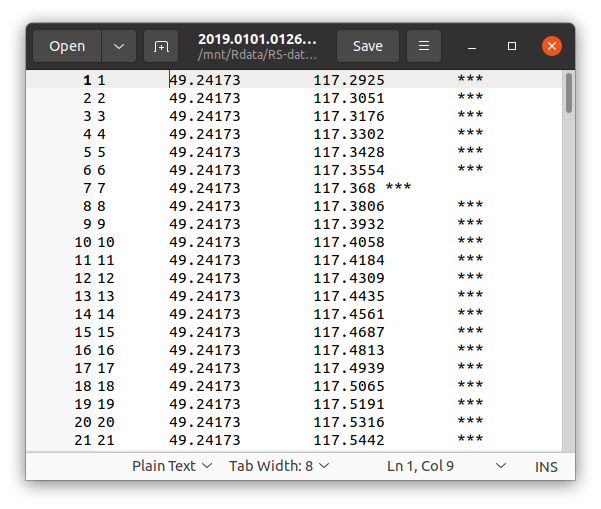
\includegraphics[scale=.6]{asc_file1}}
	\caption{NOAA/AVHRR SST 자료 텍스트 파일 캡처 화면.}
	\label{fig:asc_file}
\end{figure}

Terra/Aqua 위성의 MODIS를 구한 SST 자료는 HDF(Hierarchical Data Format) 형태로 배포되었다. HDF는 이름 그대로 계층적으로 구조화된 다차원 배열 데이터를 저장하기 위하여 HDF Gruop(https://www.hdfgroup.org/)에 의해 만들어진 파일 형식이다.

\newpage
\subsection{연구에 사용한 데이터}

해양위성센터에서 배포한 MODIS의 SST 데이터는 구름이 제거되지 않아서 SST 값에 심각한 오류를 포함하고 있어 사용하지 않고, NOAA/AVHRR의 SST 레벨2 자료를 이용하여 연구를 진행하였다. 

NOAA/AVHRR의 SST 레벨2 자료는 앞서 언급한 것 처럼 텍스트 파일 형태로 제공되고 있고, Figure \ref{fig:SST-KOSC}\와 같이 지도 위에 표출된 자료도 함께 제공되고 있다. 

\begin{figure}[htbp]
	\centerline{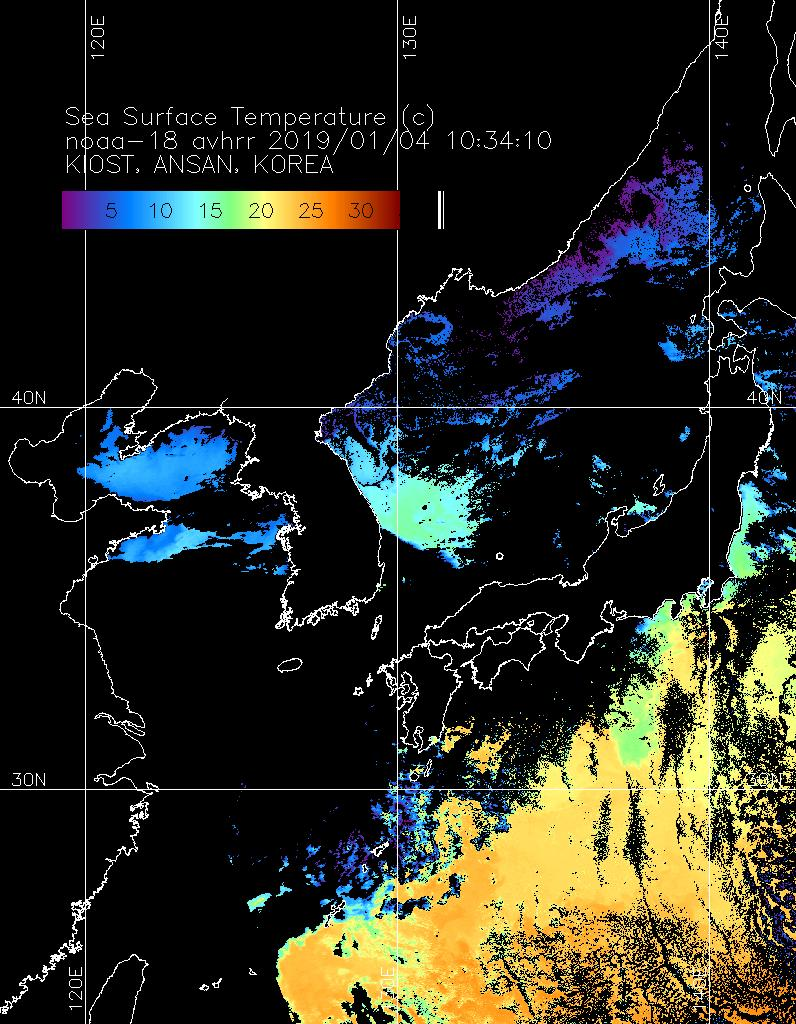
\includegraphics[width=10cm]{2019.0104.1034.noaa-18.sst}}
	\caption{KOSC에서 배포한 NOAA/AVHRR SST 자료.}
	\label{fig:SST-KOSC}
\end{figure}

KOSC로 부터 다운받아 본 연구에 사용한 NOAA/AVHRR의 SST 자료의 정보는 Table \ref{table:NOAA-data}\와 같다.

\begin{table}[!htbp]
	\caption{사용한 NOAA/AVHRR SST data.}

	\begin{tabular}{c|c|c|c|c|c}
		\hline
		
		\hline
		year   & NOAA-15 & NOAA-16 & NOAA-17 & NOAA-18 & NOAA-19 \\ 
		
		\hline
		
		\hline
		2011 & 0       & 406     & 18      & 412     & 413     \\ \hline
		2012 & 12      & 1,184   & 11      & 1,073   & 1,141   \\ \hline
		2013 & 0       & 1,229   & 0       & 1,085   & 1,145   \\ \hline
		2014 & 0       & 533     & 0       & 1,056   & 728     \\ \hline
		2015 & 0       & 0       & 0       & 1,106   & 452     \\ \hline
		2016 & 0       & 0       & 0       & 1,022   & 1,177   \\ \hline
		2017 & 0       & 0       & 0       & 818     & 1,072   \\ \hline
		2018 & 0       & 0       & 0       & 912     & 937     \\ \hline
		2019 & 0       & 0       & 0       & 847     & 843     \\ \hline
		2020 & 0       & 0       & 0       & 526     & 527     \\ 
		
		\hline

		\hline
	\end{tabular}
	\label{table:NOAA-data}
\end{table}


\newpage
\subsection{자료 처리}

NOAA/AVHRR의 SST 레벨2 자료를 위도, 경도 구간을 나눈 후, 일평균값, 주평균값, 월평균값을 산출하여 레벨3 자료를 만들었다. 자료 처리는 Phthon을 이용하여 실시하였다. 


	\section{Test Section}

Title : 21pt, bold face.

\subsection{Test Subsection}

Title : 16pt, bold face.

\subsubsection{Test Subsubsection}

Title : 14pt, normal style.

앞서 언급하였듯이 subsubsection, paragraph 와 같은 하위 절은 사용을 자제하는 것이 좋다.

\paragraph{Test Paragraph}

Title : 12pt, italic style. No numbering.
	% Next Section (e.g. Experiment, Linear theory, etc...) 
	% 이외에도 추가로 section마다 파일을 sub 폴더 안에 넣고 여기에서 
	% include 해주면 됩니다.
	% 예시 : methodology.tex을 sub 폴더안에 저장, 이 자리에 
	% \section{연구 방법 및 과정}

\subsection{데이터 파악}

해양위성센터에서 제공하는 SST 데이터를 다운받을 수 있는 경로를 확인하였다. 접근할 수 있는 데이터는 2020년 4월 29일 기준으로 Table \ref{table:KOSC-SST-data}\와 같다.


\begin{table}[!htbp]
	\caption{해양위성센터에서 다운로드 가능한 SST 데이터.}
	\begin{tabular}{c|c|c}
		\toprule
		센서명           & 자료시작시기       & 자료종료시기 (2020. 4. 29. 기준) \\ \toprule
		AVHRR         & 2011. 9. 1.  & 2020. 4. 21.          \\ \hline
		MODIS (Aqua)  & 2011. 9. 1.  & 2020. 4. 6.           \\ \hline
		MODIS (Terra) & 2011. 9. 1.  & 2020. 4. 7.           \\ \hline
		VIIRS         & 2016. 6. 17. & 2020. 4. 27.          \\ \bottomrule
	\end{tabular}

	\label{table:KOSC-SST-data}
\end{table}

NOAA/AVHRR 자료는 Fig. \ref{fig:asc_file}\와 같이 텍스트 파일의 형태로 배포되고 있다는 것을 알 수 있었다. 총 4개의 열로 저장되어 있으며, 첫번째 열부터 각각 인덱스, 위도, 경도, SST 임을 알 수 있는데, 자료가 산출되지 않은 경우에 ***로 표시되어 있다.

\begin{figure}[htbp]
	\centerline{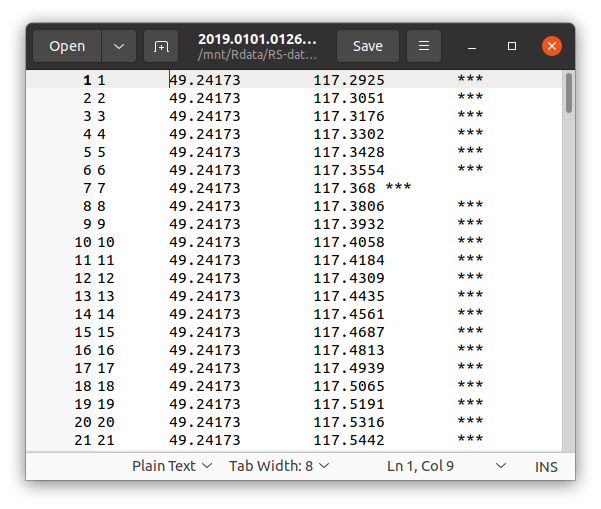
\includegraphics[scale=.6]{asc_file1}}
	\caption{NOAA/AVHRR SST 자료 텍스트 파일 캡처 화면.}
	\label{fig:asc_file}
\end{figure}

Terra/Aqua 위성의 MODIS를 구한 SST 자료는 HDF(Hierarchical Data Format) 형태로 배포되었다. HDF는 이름 그대로 계층적으로 구조화된 다차원 배열 데이터를 저장하기 위하여 HDF Gruop(https://www.hdfgroup.org/)에 의해 만들어진 파일 형식이다.

\newpage
\subsection{연구에 사용한 데이터}

해양위성센터에서 배포한 MODIS의 SST 데이터는 구름이 제거되지 않아서 SST 값에 심각한 오류를 포함하고 있어 사용하지 않고, NOAA/AVHRR의 SST 레벨2 자료를 이용하여 연구를 진행하였다. 

NOAA/AVHRR의 SST 레벨2 자료는 앞서 언급한 것 처럼 텍스트 파일 형태로 제공되고 있고, Figure \ref{fig:SST-KOSC}\와 같이 지도 위에 표출된 자료도 함께 제공되고 있다. 

\begin{figure}[htbp]
	\centerline{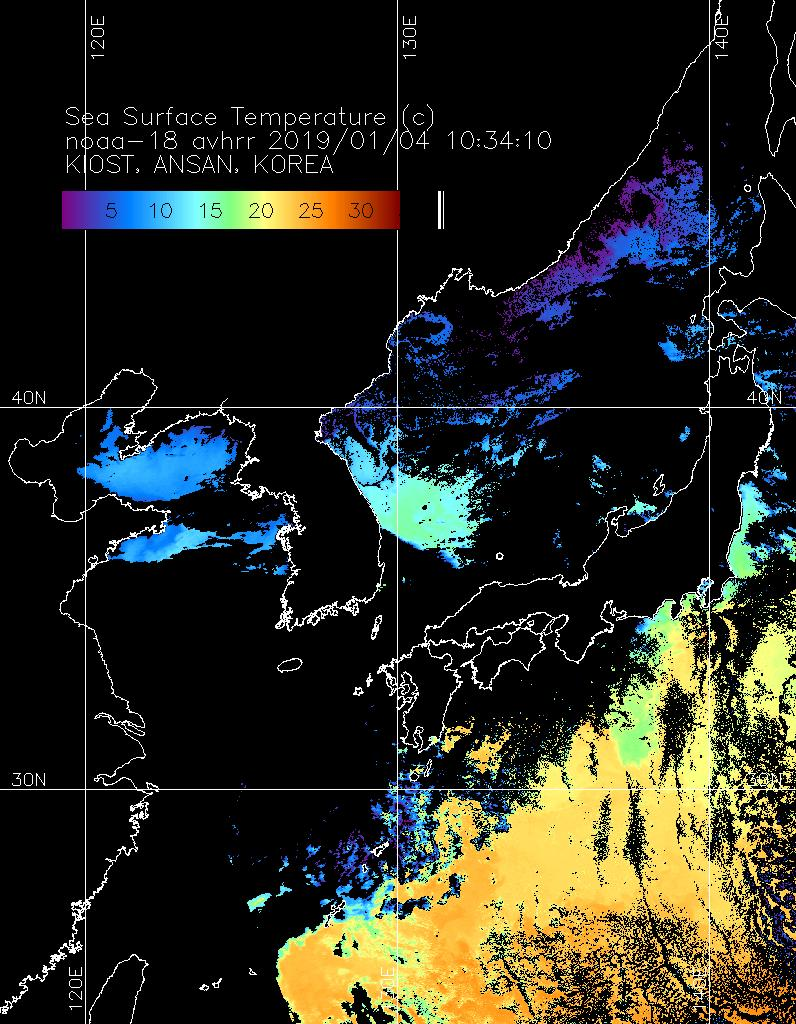
\includegraphics[width=10cm]{2019.0104.1034.noaa-18.sst}}
	\caption{KOSC에서 배포한 NOAA/AVHRR SST 자료.}
	\label{fig:SST-KOSC}
\end{figure}

KOSC로 부터 다운받아 본 연구에 사용한 NOAA/AVHRR의 SST 자료의 정보는 Table \ref{table:NOAA-data}\와 같다.

\begin{table}[!htbp]
	\caption{사용한 NOAA/AVHRR SST data.}

	\begin{tabular}{c|c|c|c|c|c}
		\hline
		
		\hline
		year   & NOAA-15 & NOAA-16 & NOAA-17 & NOAA-18 & NOAA-19 \\ 
		
		\hline
		
		\hline
		2011 & 0       & 406     & 18      & 412     & 413     \\ \hline
		2012 & 12      & 1,184   & 11      & 1,073   & 1,141   \\ \hline
		2013 & 0       & 1,229   & 0       & 1,085   & 1,145   \\ \hline
		2014 & 0       & 533     & 0       & 1,056   & 728     \\ \hline
		2015 & 0       & 0       & 0       & 1,106   & 452     \\ \hline
		2016 & 0       & 0       & 0       & 1,022   & 1,177   \\ \hline
		2017 & 0       & 0       & 0       & 818     & 1,072   \\ \hline
		2018 & 0       & 0       & 0       & 912     & 937     \\ \hline
		2019 & 0       & 0       & 0       & 847     & 843     \\ \hline
		2020 & 0       & 0       & 0       & 526     & 527     \\ 
		
		\hline

		\hline
	\end{tabular}
	\label{table:NOAA-data}
\end{table}


\newpage
\subsection{자료 처리}

NOAA/AVHRR의 SST 레벨2 자료를 위도, 경도 구간을 나눈 후, 일평균값, 주평균값, 월평균값을 산출하여 레벨3 자료를 만들었다. 자료 처리는 Phthon을 이용하여 실시하였다. 

 와 같이 작성
	%%%% 주의
	%%%% 파일이 나뉠 때마다 자동으로 페이지넘김(\clearpage)가 됩니다. 
	%%%% 따라서 subsection을 나누는 용도로는 사용하지 마십시오.
	%%%% \include{sub/experiment} 와 같이...


	\section{결론}
글이라는 것은 개인의 개성이 담겨 있기 때문에 모든 사람들이 동일한 방식으로 표현하는 것은 아니다. 그러나 고대로부터 개인의 연구 내용을 글로써 타인에게 전달할 때, 효율적인 방법이라고 공감대를 형성하며 다듬어져 온 것이 지금의 논문 형태이다. 그러므로 처음 논문을 작성하는 학생들은 이 문서에서 지시하는 논문 작성 방식을 따르는 것을 권한다. 하지만 여기서는 다양한 논문들에 대해 일일이 사례를 들어 올바른 논문 작성법을 설명하기에는 한계가 있기에 간략하게만 소개를 했다. 여기서 설명되지 않은 부분들은 다른 사람들의 논문을 참고하자. 이미 서론을 작성하면서 많은 선행 연구 논문들을 읽어 봤을 것이다. 그 논문들에서는 데이터를 어떤 방식으로 표현하는지, 서론은 어떤 흐름으로 구성하는지 등을 살펴보자. 논문을 잘 쓰는 비결의 첫 번째는 논문을 많이 읽어 보는 것이다. 

+ 첨언을 하자면, 본교의 영어논문작성법 수업에 사용되는 `Science Research Writing for Non-Native Speakers of English' 를 참고하면 많은 도움이 될 것이다. % Conclusion
	
	%\clearpage  %%% Appendix를 새 페이지에서 시작
%\appendix

\section{부록}

자료 처리에 사용한 Python 코드를 부록으로 나타내었다. 

모든 코드는 깃헙(https://github.com/guitar79/MODIS\_hdf\_Python.git)에 공유되어 있다.

\subsection{MODIS\_hdf\_utilities.py}

\lstinputlisting[language=Python]{MODIS_hdf_Python/MODIS_hdf_utilities.py}

\subsection{1.daily\_classify\_using\_AVHRR\_asc\_SST.py}
\lstinputlisting[language=Python]{MODIS_hdf_Python/1.daily_classify_using_AVHRR_asc_SST.py}

\subsection{2.statistics\_AVHRR\_asc\_SST\_alldata\_and\_creating\_NCfile.py}
\lstinputlisting[language=Python]{MODIS_hdf_Python/2.statistics_AVHRR_asc_SST_alldata_and_creating_NCfile.py}

\subsection{4.draw\_HIST\_and\_MAP\_statistics\_AVHRR\_asc\_SST\_NCfile.py}
\lstinputlisting[language=Python]{MODIS_hdf_Python/4.draw_HIST_and_MAP_statistics_AVHRR_asc_SST_NCfile.py}

 % Appendix가 없는 경우 주석처리하십시오
	
	\bibliography{bibfile} % 참고문헌
	% BibTeX 코드 쉽게 얻어오는 방법 %
	% Google Scholar 에서 검색한 결과에서 `인용'을 클릭한다.
	% BibTeX 코드를 얻고자 한다면, 하단의 `BibTeX' 을 클릭.
	% 코드가 나온다. Ctrl+A, Ctrl+C로 복사, bibfile에 붙여넣기.
	
	%\begin{summary}
\addcontentsline{toc}{section}{Summary}  %%% TOC에 표시
한글로 졸업논문을 작성한 학생은 반드시 5페이지 내외의 영어 요약문을 작성해야 합니다. 영문으로 작성하는 학생은 이 부분을 작성하지 않아도 됩니다.
\end{summary} % Summary
	%(영어로 작성한 학생은 이 부분을 주석 처리하십시오.)
	
	%%-----------------------------------------------------
%   감사의 글
%-----------------------------------------------------
\begin{acknowledgements}
\addcontentsline{toc}{section}{감사의 글}  %%% TOC에 표시
정말 감사합니다.
\end{acknowledgements}

%-----------------------------------------------------
%   연구활동 
%-----------------------------------------------------
\begin{researches}
\addcontentsline{toc}{section}{연구활동}  %%% TOC에 표시
\begin{itemize}
\item{2011학년도 교내 R\&E 발표대회에서 장려상 수상}
\item{2012학년도 교내 R\&E 발표대회에서 장려상 수상}
\item{2013학년도 교내 R\&E 발표대회에서 장려상 수상}
\item{2014학년도 교내 R\&E 발표대회에서 장려상 수상}
\item{2015학년도 교내 R\&E 발표대회에서 장려상 수상}
\item{2016학년도 교내 R\&E 발표대회에서 장려상 수상}
\item{2017학년도 교내 R\&E 발표대회에서 장려상 수상}
\item{2018학년도 교내 R\&E 발표대회에서 장려상 수상}
\item{2019년 노벨 물리학상 수상}
\end{itemize}
\end{researches} % 감사의 글 & 연구활동
\end{document}
